\documentclass[../main.tex]{subfiles}

\begin{document}


\practica{7}{Buses de Expansión - I2C y pantalla táctil}

    \subsection{Objetivos}
        \begin{itemize}
            \item Entender el funcionamiento básico del bus I2C.
            \item Programar un driver para la comunicación con la pantalla táctil a través de I2C.
        \end{itemize}

    \subsection{Fundamentos teóricos}
        
        Los procesadores tienen, por regla general, un gran número de pines disponibles para su conexión con dispositivos externos (de hecho, cuentan con varios miles en los modelos más avanzados). Sin embargo, esta disponibilidad tiene sus limitaciones: en primer lugar, no todos los pines son capaces de realizar todas las funciones. En segundo lugar, el uso de pines concretos requiere un grado de planificación del sistema completo a nivel de placa base. 
        
        Mucha veces querremos la posibilidad de conectar diferentes dispositivos a nuestro diseño, pero no necesariamente que éstos existan desde el comienzo. Por ejemplo, un microcontrolador sencillo puede utilizarse para controlar diferentes tipos de sensores, actuadores, pantallas, controles y, a nivel de diseño, sólo podremos ofrecer unos pocos pines al usuario.

        Para tener la posibilidad de conectar multitud de dispositivos a nuestro procesador, existe el concepto de bus: protocolos que utilizan un conjunto reducido de pines, y permiten, a través de unas pocas líneas de datos, la interconexión de varios (en ocasiones hasta cientos) dispositivos.

        El \textbf{Bus I2C} (\emph{Inter-Integrated Circuit} es una de estas alternativas. Es de las más sencillas, y permite, a través de únicamente dos líneas, la conexión de hasta 1000 dispositivos. Los elementos más destacables del bus I2C pueden verse en la \Cref{fig:i2c_bus} y son:

        \begin{figure}[hb]
            \centering
            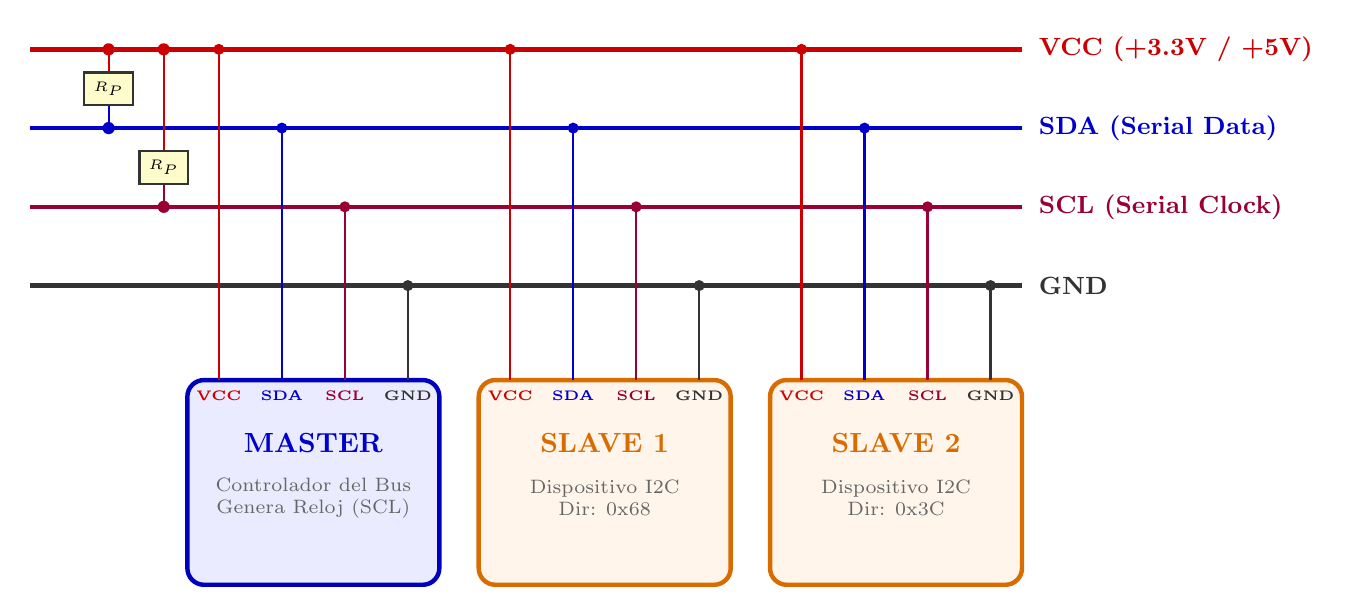
\begin{tikzpicture}[
                font=\sffamily\small,
                % Estilos de los bloques
                master box/.style={
                    draw=blue!75!black,
                    fill=blue!8,
                    ultra thick,
                    rounded corners=6pt,
                    minimum width=3.2cm,
                    minimum height=2.6cm
                },
                slave box/.style={
                    draw=orange!85!black,
                    fill=orange!8,
                    ultra thick,
                    rounded corners=6pt,
                    minimum width=3.2cm,
                    minimum height=2.6cm
                },
                resistor/.style={
                    draw=black!80,
                    fill=yellow!20,
                    thick,
                    minimum width=0.35cm,
                    minimum height=0.35cm,
                    font=\tiny\bfseries
                },
                pin label/.style={
                    font=\tiny\bfseries,
                    inner sep=1pt
                }
            ]

                % --- COORDENADAS Y DE LAS LÍNEAS DEL BUS ---
                \def\yVCC{4.2}
                \def\ySDA{3.2}
                \def\ySCL{2.2}
                \def\yGND{1.2}

                \def\xStart{-0.8}
                \def\xEnd{11.8}

                % --- LÍNEAS PRINCIPALES DEL BUS ---
                \draw[red!80!black, ultra thick] (\xStart, \yVCC) -- (\xEnd, \yVCC) node[right=2pt, font=\bfseries\small] {VCC (+3.3V / +5V)};
                \draw[blue!80!black, ultra thick] (\xStart, \ySDA) -- (\xEnd, \ySDA) node[right=2pt, font=\bfseries\small] {SDA (Serial Data)};
                \draw[purple!80!black, ultra thick] (\xStart, \ySCL) -- (\xEnd, \ySCL) node[right=2pt, font=\bfseries\small] {SCL (Serial Clock)};
                \draw[black!80, ultra thick] (\xStart, \yGND) -- (\xEnd, \yGND) node[right=2pt, font=\bfseries\small] {GND};

                % --- RESISTENCIAS DE PULL-UP (I2C Open-Drain) ---
                \def\xRone{0.2}
                \def\xRtwo{0.9}

                % Pull-up para SDA
                \node[resistor] (R1) at (\xRone, \ySDA + 0.5) {$R_P$};
                \draw[red!80!black, thick] (\xRone, \yVCC) -- (R1.north);
                \draw[blue!80!black, thick] (R1.south) -- (\xRone, \ySDA);
                \fill[red!80!black] (\xRone, \yVCC) circle (2.2pt);
                \fill[blue!80!black] (\xRone, \ySDA) circle (2.2pt);

                % Pull-up para SCL
                \node[resistor] (R2) at (\xRtwo, \ySCL + 0.5) {$R_P$};
                \draw[red!80!black, thick] (\xRtwo, \yVCC) -- (R2.north);
                \draw[purple!80!black, thick] (R2.south) -- (\xRtwo, \ySCL);
                \fill[red!80!black] (\xRtwo, \yVCC) circle (2.2pt);
                \fill[purple!80!black] (\xRtwo, \ySCL) circle (2.2pt);

                % --- DISPOSITIVOS (MASTER Y SLAVES) ---
                % Master
                \def\xM{2.8}
                \node[master box] (master) at (\xM, -1.3) {};
                \node[font=\bfseries, color=blue!80!black] at (\xM, -0.8) {MASTER};
                \node[align=center, font=\scriptsize, color=gray!80!black] at (\xM, -1.5) {Controlador del Bus\\Genera Reloj (SCL)};

                % Slave 1
                \def\xSone{6.5}
                \node[slave box] (slave1) at (\xSone, -1.3) {};
                \node[font=\bfseries, color=orange!85!black] at (\xSone, -0.8) {SLAVE 1};
                \node[align=center, font=\scriptsize, color=gray!80!black] at (\xSone, -1.5) {Dispositivo I2C\\Dir: 0x68};

                % Slave 2
                \def\xStwo{10.2}
                \node[slave box] (slave2) at (\xStwo, -1.3) {};
                \node[font=\bfseries, color=orange!85!black] at (\xStwo, -0.8) {SLAVE 2};
                \node[align=center, font=\scriptsize, color=gray!80!black] at (\xStwo, -1.5) {Dispositivo I2C\\Dir: 0x3C};

                % --- CONEXIONES DE PIN PREDETERMINADAS ---
                \foreach \xDev in {\xM, \xSone, \xStwo} {
                    \def\xVccPin{\xDev - 1.2}
                    \def\xSdaPin{\xDev - 0.4}
                    \def\xSclPin{\xDev + 0.4}
                    \def\xGndPin{\xDev + 1.2}
                    \def\yTop{0.0}

                    % Conexiones verticales a los buses
                    \draw[red!80!black, thick] (\xVccPin, \yTop) -- (\xVccPin, \yVCC);
                    \draw[blue!80!black, thick] (\xSdaPin, \yTop) -- (\xSdaPin, \ySDA);
                    \draw[purple!80!black, thick] (\xSclPin, \yTop) -- (\xSclPin, \ySCL);
                    \draw[black!80, thick] (\xGndPin, \yTop) -- (\xGndPin, \yGND);

                    % Puntos de unión en el bus
                    \fill[red!80!black] (\xVccPin, \yVCC) circle (2pt);
                    \fill[blue!80!black] (\xSdaPin, \ySDA) circle (2pt);
                    \fill[purple!80!black] (\xSclPin, \ySCL) circle (2pt);
                    \fill[black!80] (\xGndPin, \yGND) circle (2pt);

                    % Etiquetas de los pines dentro de las cajas
                    \node[pin label, red!80!black] at (\xVccPin, -0.2) {VCC};
                    \node[pin label, blue!80!black] at (\xSdaPin, -0.2) {SDA};
                    \node[pin label, purple!80!black] at (\xSclPin, -0.2) {SCL};
                    \node[pin label, black!80] at (\xGndPin, -0.2) {GND};
                }

            \end{tikzpicture}
            \caption{Diagrama de un bus I2C}
            \label{fig:i2c_bus}
        \end{figure}

        \begin{itemize}
            \item \emph{Master}: Un único dispositivo que tiene el control del bus, y genera las peticiones en el mismo. El \emph{Master} puede cambiar con ciertas señalizaciones especiales, pero siempre debe ser un único dispositivo.
            \item \emph{Slave}: Pueden ser múltiples, son dispositivos que están conectados al bus y escuchan el mismo a la espera de peticiones del \emph{Master}.
            \item \textbf{SDA} o \emph{Serial Data}: Línea de datos serie, a través de la cual se envía la información (bien del \emph{Master} al \emph{Slave} o viceversa).
            \item \textbf{SCL} o \emph{Serial Clock}: Línea de reloj serie. Controlada por el \emph{Master}, lleva la señal de reloj con la que se sincronizan los datos de \textbf{SDA}. Generalmente, los dispositivos \textbf{I2C} permiten un amplio rango de frecuencias para su funcionamiento, aunque las más típicas son 100 o 400 KHz.
        \end{itemize}

        Un dato interesante a observar es el hecho de que tanto \textbf{SCL} como \textbf{SDA} tienen resistencia de \emph{pull-up} a VCC. Es decir, que por defecto están siempre a ``1''. Cualquier dispositivo que se conecte, operará en modo de \emph{colector abierto} (open drain). Es decir, que únicamente podrá bajar la línea a ``0'' conectándola a tierra, enviándose los ``unos'' pasivamente.

        \subsubsection{Funcionamiento del bus I2C - capa física}

            Una vez realizadas las conexiones entre los dispositivos, la siguiente pregunta razonable es cómo opera el bus I2C. Las transferencias de datos siguen, de manera general, los siguientes pasos:

            \begin{enumerate}
                \item Una transferencia se inicia con una condición de inicio (\textbf{S} (start)), que se señala desde el \emph{Master} bajando \textbf{SDA} a ``0'', mientras \textbf{SCL} se mantiene a ``1''.
                \item A continuación \textbf{SCL} comienza a oscilar, bajando a ``0'' en primer lugar, mientras se prepara el bit a enviar en \textbf{SDA}.
                \item Cuando \textbf{SCL} sube a 1, el bit enviado está disponible en \textbf{SDA} y el resto de dispositivos \emph{Slaves} pueden leerlo. 
                \item Se repiten los pasos 2 y 3 tantas veces sea necesario para enviar todos los bits.
                \item El último bit es seguido de un pulso de reloj sin dato, en el cual \textbf{SDA} se pone a ``0''.
                \item Finalmente, se indica la condición de fin (\textbf{P} (stop)), liberando primero \textbf{SCL}, y posteriormente \textbf{SDA}.
            \end{enumerate}

            Este proceso se puede ver gráficamente en la \Cref{fig:i2c_transfer}.
            
            \begin{figure}[h]
                \centering
                
\includegraphics[width=\textwidth]{res/I2C_data_transfer.png}
                \caption{Transferencia de datos en I2C. (fuente:wikipedia)}
                \label{fig:i2c_transfer}
            \end{figure}

        \subsubsection{Direccionamiento en I2C - capa lógica}\label{subsub:i2clogic}
            
            Ahora bien, dentro de estas transferencias, ¿cómo sabemos a qué dispositivo van los bits? para ello, cada \emph{Slave} cuenta con una dirección (de 7 bits, o 10 en versiones más modernas), habitualmente fijada por hardware, y con la que se puede identificar un dispositivo concreto. Así, para escribir, se seguirá el siguiente procedimiento:

            \begin{enumerate}
                \item Inicio de comunicación con condición inicial \textbf{S} seguida de la dirección (7 bits) + bit ``0'' (write). \emph{Slave} responde \textbf{ACK}.
                \item Envío del comando (o registro destino) (8 bits). \emph{Slave} responde \textbf{ACK}.
                \item Envío del dato (8 bits). \emph{Slave} responde \textbf{ACK}.
                \item Generalmente, y según dispositivo, se pueden enviar datos consecutivos que irán a parar a registros consecutivos si se quiere.
                \item Fin de comunicación con condición de parada \textbf{P}.
            \end{enumerate}

            Para leer, el proceso es algo más complejo, ya que primero indicaremos el registro en modo escritura, y posteriormente cederemos el control al \emph{Slave} en modo lectura para que nos pase el dato por el bus.

            \begin{enumerate}
                \item Inicio de comunicación con condición inicial \textbf{S} seguida de la dirección (7 bits) + bit ``0'' (write). \emph{Slave} responde \textbf{ACK}.
                \item Envío del comando (o registro destino) (8 bits). \emph{Slave} responde \textbf{ACK}.
                \item Re-Inicio de comunicación con condición inicial \textbf{S} seguida de la dirección (7 bits) + bit ``1'' (read). \emph{Slave} responde \textbf{ACK}.
                \item El \emph{Slave} toma el control y envía el dato de vuelta (8 bits). El \emph{Master} puede responder con \textbf{ACK} para pedir más datos consecutivos, o con \textbf{NACK} para terminar la comunicación.
                \item Fin de comunicación con condición de parada \textbf{P}.
            \end{enumerate}

            Las condiciones \textbf{ACK} y \textbf{NACK} se indican, respectivamente, con un ``0'' y un ``1'' (sí, están invertidas) por parte del receptor, en la línea \textbf{SDA} tras las transmisión de un byte.

            El proceso para ambas transacciones puede observarse en la \Cref{fig:i2c_read_write}

            \definecolor{masterBG}{HTML}{EBF5FB}
            \definecolor{masterBORDER}{HTML}{2980B9}
            \definecolor{slaveBG}{HTML}{FEF9E7}
            \definecolor{slaveBORDER}{HTML}{D68910}
            \definecolor{ctrlBG}{HTML}{FDEDEC}
            \definecolor{ctrlBORDER}{HTML}{CB4335}

            \tikzset{
                i2cbase/.style={
                    draw, 
                    minimum height=0.9cm, 
                    font=\sffamily\scriptsize, 
                    align=center, 
                    outer sep=0pt, 
                    line width=0.6pt
                },
                master/.style={i2cbase, fill=masterBG, draw=masterBORDER, text=masterBORDER!40!black},
                slave/.style={i2cbase, fill=slaveBG, draw=slaveBORDER, text=slaveBORDER!40!black},
                ctrl/.style={i2cbase, fill=ctrlBG, draw=ctrlBORDER, text=ctrlBORDER!40!black, font=\sffamily\bfseries\scriptsize},
                opt/.style={i2cbase, fill=masterBG!30, draw=masterBORDER, dashed, text=masterBORDER!40!black},
                title/.style={font=\sffamily\bfseries\small, text=gray!90!black},
                stepnum/.style={font=\sffamily\bfseries\tiny, text=gray!70!black},
                legendtext/.style={font=\sffamily\tiny, text=gray!80!black}
            }

            \begin{figure}[h!]
                \centering
                \begin{tikzpicture}
                    \node[ctrl, minimum height=0.4cm, minimum width=0.6cm] (l1) {};
                    \node[legendtext, right=3pt of l1] {Inicio / Fin (Master)};
                    
                    \node[master, minimum height=0.4cm, minimum width=0.6cm, right=100pt of l1] (l2) {};
                    \node[legendtext, right=3pt of l2] {Generado por \textbf{Master}};
                    
                    \node[slave, minimum height=0.4cm, minimum width=0.6cm, right=100pt of l2] (l3) {};
                    \node[legendtext, right=3pt of l3] {Generado por \textbf{Slave}};
                \end{tikzpicture}
                \resizebox{\linewidth}{!}{%
                \begin{tikzpicture}[node distance=0pt]

                    % Título del diagrama
                    \node[title, anchor=west] (t1) at (0, 1.3) {1. Escritura en I2C (Write)};

                    % Bloques del protocolo de escritura
                    \node[ctrl, minimum width=0.6cm] (w_s) at (0,0) {\textbf{S}};
                    \node[master, right=-0.6pt of w_s, minimum width=1.8cm] (w_addr) {Dirección Slave\\(7 bits)};
                    \node[master, right=-0.6pt of w_addr, minimum width=0.7cm] (w_bit) {0\\(W)};
                    \node[slave, right=-0.6pt of w_bit, minimum width=0.9cm] (w_ack1) {\textbf{ACK}\\(0)};
                    \node[master, right=-0.6pt of w_ack1, minimum width=2.2cm] (w_reg) {Registro / Cmd\\(8 bits)};
                    \node[slave, right=-0.6pt of w_reg, minimum width=0.9cm] (w_ack2) {\textbf{ACK}\\(0)};
                    \node[master, right=-0.6pt of w_ack2, minimum width=1.8cm] (w_data) {Dato\\(8 bits)};
                    \node[slave, right=-0.6pt of w_data, minimum width=0.9cm] (w_ack3) {\textbf{ACK}\\(0)};
                    \node[opt, right=-0.6pt of w_ack3, minimum width=1.8cm] (w_dataN) {Dato N (opc.)\\(8 bits)};
                    \node[slave, right=-0.6pt of w_dataN, minimum width=0.9cm] (w_ackN) {\textbf{ACK}\\(0)};
                    \node[ctrl, right=-0.6pt of w_ackN, minimum width=0.6cm] (w_p) {\textbf{P}};

                    % Indicadores de pasos
                    \node[stepnum, above=3pt of w_s] {Paso 1};
                    \node[stepnum, above=3pt of w_addr] {Paso 2};
                    \node[stepnum, above=3pt of w_reg] {Paso 3};
                    \node[stepnum, above=3pt of w_data] {Paso 4};
                    \node[stepnum, above=3pt of w_dataN] {Paso 5};
                    \node[stepnum, above=3pt of w_p] {Paso 6};

                \end{tikzpicture}%
                }
                \vspace{0.8cm}
                \resizebox{\linewidth}{!}{%
                \begin{tikzpicture}[node distance=0pt]

                    % Título del diagrama
                    \node[title, anchor=west] (t2) at (0, 1.3) {2. Lectura en I2C (Read)};

                    % Bloques del protocolo de lectura
                    \node[ctrl, minimum width=0.6cm] (r_s) at (0,0) {\textbf{S}};
                    \node[master, right=-0.6pt of r_s, minimum width=1.7cm] (r_addr1) {Dirección Slave\\(7 bits)};
                    \node[master, right=-0.6pt of r_addr1, minimum width=0.6cm] (r_w) {0\\(W)};
                    \node[slave, right=-0.6pt of r_w, minimum width=0.8cm] (r_ack1) {\textbf{ACK}\\(0)};
                    \node[master, right=-0.6pt of r_ack1, minimum width=2.0cm] (r_reg) {Registro / Cmd\\(8 bits)};
                    \node[slave, right=-0.6pt of r_reg, minimum width=0.8cm] (r_ack2) {\textbf{ACK}\\(0)};
                    \node[ctrl, right=-0.6pt of r_ack2, minimum width=0.6cm] (r_sr) {\textbf{Sr}};
                    \node[master, right=-0.6pt of r_sr, minimum width=1.7cm] (r_addr2) {Dirección Slave\\(7 bits)};
                    \node[master, right=-0.6pt of r_addr2, minimum width=0.6cm] (r_r) {1\\(R)};
                    \node[slave, right=-0.6pt of r_r, minimum width=0.8cm] (r_ack3) {\textbf{ACK}\\(0)};
                    \node[slave, right=-0.6pt of r_ack3, minimum width=1.8cm] (r_data) {Dato Slave\\(8 bits)};
                    \node[master, right=-0.6pt of r_data, minimum width=1.0cm] (r_nack) {\textbf{NACK}\\(1)};
                    \node[ctrl, right=-0.6pt of r_nack, minimum width=0.6cm] (r_p) {\textbf{P}};

                    % Indicadores de pasos
                    \node[stepnum, above=3pt of r_s] {Paso 1};
                    \node[stepnum, above=3pt of r_addr1] {Paso 2};
                    \node[stepnum, above=3pt of r_reg] {Paso 3};
                    \node[stepnum, above=3pt of r_sr] {Paso 4};
                    \node[stepnum, above=3pt of r_addr2] {Paso 5};
                    \node[stepnum, above=3pt of r_data] {Paso 6};
                    \node[stepnum, above=3pt of r_p] {Paso 7};

                \end{tikzpicture}%
                }
                \caption{Escrituras y lecturas, respectivamente, en I2C}
                \label{fig:i2c_read_write}
            \end{figure}
                    
        \subsubsection{Líneas auxiliares a I2C}

            En ocasiones, utilizar únicamente las líneas \textbf{SCL} y \textbf{SDA} no es suficiente. Pensemos por ejemplo en el caso de las interrupciones. Con tan sólo las dos líneas de I2C, capturar una interrupción es imposible, tendríamos que hacer una encuesta activa a los periféricos, preguntando periódicamente si tienen algún dato de interés. Esto sería claramente ineficiente.

            Es por ello que las interrupciones de los dispositivos sí van por líneas separadas, para que el procesador sea capaz de capturarlas, identificar directamente el dispositivo causante, y entonces, y sólo entonces, encuestarlo vía I2C para recibir el dato. Es el caso, por ejemplo, con nuestra pantalla táctil y la detección de pulsaciones.

            Adicionalmente, algunos dispositivos disponen de señales extra, para habilitarlos o resetearlos.

        \subsubsection{Conexiones en nuestra placa}

            Podemos ver el pinout completo de las conexiones procesador-pantalla táctil en \BRDMAN[6.8]. El conector a la pantalla táctil tiene señales \textbf{SCL}, \textbf{SDA}, \textbf{INT}, \textbf{RESET}, además de varias conexiones para alimentación y tierra. Estas últimas son pasivas y no requieren de control por parte del procesador.

            Las que sí requieren de control, se especifican en \BRDMAN[Appendix A]. Ahí, podemos ver las conexiones que se especifican en la \Cref{tab:ctp_conn}

            \begin{table}[h]
                \centering
                \begin{tabular}{c|c|c}
                    Pin & Function & Connection \\\hline\hline
                    PA8 & I2C3 SCL & CTP SCL \\
                    PH8 & I2C3 SDA & CTP SDA \\
                    PH9 & GPIO OUTPUT & CTP RST \\ 
                    PI9 & GPIO EXTI9 & CTP INT \\
                \end{tabular}
                \caption{Conexiones para la pantalla. CTP: \emph{Connector Touch Panel}. Los pines PA8 y PH8 no vienen completamente especificados en \BRDMAN, pero se incluyen aquí por completitud.}
                \label{tab:ctp_conn}
            \end{table}

    \subsection{Desarrollo de la práctica}

        Llegados a este punto, y con la teoría del bus I2C vista, sólo nos queda comunicarnos con el panel táctil. Haremos una aplicación donde el usuario ``pintará'' con el dedo en la pantalla. Para ello, partiremos de la práctica anterior, donde ya teníamos el controlador de la pantalla funcionando. En lugar de pintarse aleatoriamente, ahora controlaremos nosotros el pintado. Para ello, habrá que hacer lo siguiente:

        \begin{itemize}
            \item Configurar el bus I2C para poder comunicarnos con el panel táctil (CTP).
            \item Activar las interrupciones adecuadas para recibir eventos del CTP.
            \item Crear el driver que nos permita leer los eventos y transformarlos a coordenadas para pintar en la pantalla.
        \end{itemize}

        Vamos por orden:

        \subsubsection{Configuración del bus I2C}
            
            Lo primero que debemos hacer es activar los pines adecuados para la comunicación. En primer lugar, los pines \textbf{SCL} y \textbf{SDA} (PA8 y PH8) deben configurarse en modo alternativo con función 4 (esto los conecta al I2C3, ver \DSMAN[Table 12]), modo open drain, sin pull up y velocidad alta. Además, hay que asegurarse de activar \REG{GPIOAEN} y \REG{GPIOBEN} en \REG{AHB1ENR} (\REFMAN[5.3.10]).

            Por otro lado, debemos asegurarnos que el CTP no está en modo RESET, para ello, debemos activar el GPIO para el pin PH9 (Correspondiente a CTP RESET (\Cref{tab:ctp_conn})). Este pin debe configurarse en modo salida, push-pull sin pullup, y velocidad baja. A continuación debemos escribir un ``1'' en él para desactivar el RESET (que es en lógica inversa).

            \begin{lstlisting}
                void I2C3_Pins_Init() {
                    //Pin A8 has I2C_SCL
                    // ... completar
                    //Pin H8 has I2C_SDA
                    // ... completar
                    //Pin H9 para el reset del CTP
                    // ... completar
                }         
            \end{lstlisting}

            Con esto los pines ya están activos, y nos toca configurar el periférico I2C. Las definiciones de los registros que contiene se pueden ver en \REFMAN[26.9], y la dirección base se puede encontrar en \REFMAN[1.6.2]. Se ofrece a continuación el código para \texttt{bsp.h} con las definiciones y algunas funciones predefinidas creadas:

            \begin{lstlisting}
                #define I2C3_BASE_ADDR 0x40005C00UL

                typedef struct
                {
                    volatile uint32_t CR1;      /* Control register 1,            */
                    volatile uint32_t CR2;      /* Control register 2,            */
                    volatile uint32_t OAR1;     /* Own address 1 register,        */
                    volatile uint32_t OAR2;     /* Own address 2 register,        */
                    volatile uint32_t TIMINGR;  /* Timing register,               */
                    volatile uint32_t TIMEOUTR; /* Timeout register,              */
                    volatile uint32_t ISR;      /* Interrupt and status register, */
                    volatile uint32_t ICR;      /* Interrupt clear register,      */
                    volatile uint32_t PECR;     /* PEC register,                  */
                    volatile uint32_t RXDR;     /* Receive data register,         */
                    volatile uint32_t TXDR;     /* Transmit data register,        */
                } I2C_TypeDef;

                #define I2C3				((I2C_TypeDef *) I2C3_BASE_ADDR)
                
                static inline void I2C_Disable(I2C_TypeDef * I2Cx) {
                    I2Cx->CR1 &= ~(0x1);
                }

                static inline void I2C_Enable(I2C_TypeDef * I2Cx) {
                    I2Cx->CR1 |=  (0x1);
                }

                static inline void I2C_Set_Timing(I2C_TypeDef * I2Cx, uint32_t presc, uint32_t scldel, uint32_t sdadel, uint32_t sclh, uint32_t scll) {
                    I2Cx->TIMINGR = (presc << 28) | (scldel << 20) | (sdadel << 16) | (sclh << 8) | (scll);
                }
            \end{lstlisting}

            En lo que a nosotros respecta, debemos utilizar estas funciones para inicializar el periférico \PER{I2C3} (\REFMAN{26}). En \REFMAN[26.4.5], tenemos un diagrama que nos indica cómo proceder para configurar el controlador I2C. Como no necesitamos todas las funciones, lo haremos algo más sencillo. 

            Lo primero será activar el periférico \PER{I2C3} desde \REG{APB1ENR} (\REFMAN[5.3.13]), para a continuación aplicar una secuencia de reseteo desde \REG{APB1RST} (\REFMAN[5.3.8]) consistente en escribir un 1 y luego un 0 sobre el bit de \PER{I2C3}. Tras esto, ya podemos configurar el periférico. Para ello se inhabilita (ya desde dentro de su registro \REG{I2C\_CR1}), se configura el temporizador \REG{I2C\_TIMINGR}, y se vuelve a habilitar.

            Para la temporización, hay numerosos campos. Tenemos que configurarlos teniendo en cuenta que la frecuencia base son 16MHz. La frecuencia objetivo que queremos son 400KHz. Hay muchas maneras de conseguirla, tenemos que tener en cuenta que la fórmula es la siguiente:

            \[
                f_{obj} = \frac{f_{base}}{(PRESC+1)*(SCLL+1+SCLH+1)}
            \]

            \REG{SCLL} y \REG{SCLH} indican el tiempo que la señal de reloj pasará, respectivamente, a baja (low) y alta (high). Podemos ponerlos iguales para conseguir una señal cuadrada. El valor de \REG{PRESC} es un preescaler que nos divide la señal de reloj por si fuera muy alta. En nuestro caso, podemos dejar el prescaler a 0, y poner los otros dos registros a 19, para conseguir una onda cuadrada exacta a 400KHz. Los valores de \REG{SCLDEL} y \REG{SDADEL} controlan los desfases entre las subidas y bajadas de \textbf{SCL} y \textbf{SDA}. En general son valores bastante flexibles, aunque sus detalles son complejos y pueden explorarse más en \REFMAN[26.9.5] y \REFMAN[26.4.5]. Para nuestro caso, con 3 y 1 respectivamente debería funcionar.

            \begin{lstlisting}
                void I2C3_Reg_Config() {
                    //Enable I2C3 and reset cycle 
                    // ... completar

                    //Configure I2C
                    I2C_Disable(I2C3);
                    // Set Timing 
                    // ... completar 
                    I2C_Enable(I2C3);
                }
            \end{lstlisting}

        \subsubsection{Interrupciones del CTP}

            A continuación debemos activar las interrupciones del panel táctil. Como vimos en \Cref{tab:ctp_conn} tiene un pin dedicado para interrumpir al procesador, a través de la línea de interrupción externa \texttt{EXTI9}. Debemos configurar el procesador para atender esa petición. Recordemos que cada línea de interrupción externa \texttt{EXTIx} puede conectarse a cualquiera de los puertos (PA, PB, \dots) \REFMAN[10]. En este caso, como interrumpimos desde \texttt{PI9}, debemos configurar \texttt{EXTI9} para que atienda al puerto \texttt{I} en modo falling edge. Además, debemos indicar desde \PER{SYSCFG} en el registro \REG{EXTICR} (\REFMAN[7.2.3]) que el puerto I (\texttt{8}) es el que se atiende en \texttt{EXTI9}, y activar \PER{SYSCFG} desde el bit de enable de \REG{APB2ENR} (\REFMAN[5.3.19]). Finalmente, tenemos que activar la interrupción correspondiente en el \PER{NVIC} (\REFMAN[9.1.2]).

            Hay que tener en cuenta que las interrupciones externas están agrupadas (en concreto, de la 5 a la 9 se atienden juntas (\REFMAN[9.1.2]) a través de la línea de interrupción número 23 del procesador). Así que, en nuestra rutina de interrupción, tendremos que asegurarnos de que fue la interrupción externa 9 la que causó la interrupción a través del registro \REG{PR} de \PER{EXTI} (\REFMAN[10.9.6])

            \begin{lstlisting}
                void TS_INT_Init(void) {
                    // ... completar activar GPIO PI9 como entrada pull-up, velocidad rápida
                    
                    /* Enable and Map EXTI Line 9 to GPIOI (0b1000 = Port I) */
                    // ... completar activar SYSCFGEN en APB2ENR
                    // ... configurar int 9 para atenderse desde PI en EXTICR
                    // ... activar interrupción EXTI9 en EXTI
                    // ... habilitar modo falling edge y deshabilitar rising edge
                    // ... activar interupción 23 (EXTI9_5) en NVIC
                }

                void EXTI9_5_IRQHandler(void) {
                    // ... completar comprobar bit 9 de EXTI PR
                    if () {
                        // ... limpiar bit 9 de EXTI PR
                        g_ts_interrupt_flag = 1;	// Notify main thread
                    }
                }
            \end{lstlisting}

            Con esto, ya tendremos las interrupciones disparando ante eventos del panel táctil. De hecho, puedes probar a ejecutar el código con un \emph{breakpoint} en la interrupción, y deberías ver que se dispara al tocar la pantalla, aunque no recojamos dato alguno.

        \subsubsection{Driver del I2C}

            Nos falta leer los datos correspondientes a la posición, y hacer algo con ellos. Para ello necesitamos dos cosas: 

            \begin{itemize}
                \item Un \emph{driver} para el periférico \PER{I2C} que nos permita leer/escribir a través del bus (programaremos ambas funciones, aunque sólo utilizaremos la primera).
                \item Otro \emph{driver} que, utilizando el primero, se comunique con el panel táctil para leer la posición de la pulsación.
            \end{itemize}

            Lo primero de todo es crear el driver para \PER{I2C} (\REFMAN[26]). Vamos a empezar por unas cuantas funciones auxiliares para el control de los diversos registros internos. Analízalas bien, viendo los registros que utilizan y el manual, para comprender su funcionamiento:

            \begin{lstlisting}
                static inline void I2C_Write(I2C_TypeDef *I2Cx, uint8_t data) {
                    // Wait for TXDR to be empty (TXIS == 0)
                    while (!(I2Cx->ISR & (1U << 1U)));
                    // Load byte into Transmit Data Register
                    I2Cx->TXDR = data;
                }

                static inline uint8_t I2C_Read(I2C_TypeDef *I2Cx) {
                    // Wait for RXNE (Receive Buffer Not Empty flag)
                    while (!(I2Cx->ISR & (1U << 2U)));
                    // Read byte from Receive Data Register
                    return (uint8_t)(I2Cx->RXDR & 0xFFU);
                }

                static inline void I2C_Wait_TC(I2C_TypeDef *I2Cx) {
                    // Wait for TC (Transfer Complete flag)
                    while (!(I2Cx->ISR & (1U << 6U)));
                }

                static inline void I2C_Stop(I2C_TypeDef *I2Cx) {
                    // Generate STOP condition (STOP bit 14 in CR2)
                    I2Cx->CR2 |= (1U << 14U);
                    // Wait for STOPF (Stop detection flag bit 5 in ISR)
                    while (!(I2Cx->ISR & (1U << 5U)));
                    // Clear STOPF flag by writing to ICR (STOPCF bit 5 in ICR)
                    I2Cx->ICR |= (1U << 5U);
                }
            \end{lstlisting}

            Uno de los registros más importantes es \REG{CR2} (\REFMAN[26.9.2]). Nos va a permitir configurar la transferencia que queremos realizar (dirección destino, número de bytes a trasferir, si es escritura o lectura, y algunas funciones más que no utilizaremos). Estúdialo bien, e implementa la función \texttt{I2C\_Start}:

            \begin{lstlisting}
                typedef enum {
                    I2C_WRITE = 0U,
                    I2C_READ  = 1U
                } I2C_Direction;

                static inline void I2C_Start(I2C_TypeDef *I2Cx, uint8_t slave_addr, I2C_Direction direction, uint32_t len) {
                    uint32_t cr2 = 0;

                    // ... completar Set 7-bit Slave Address (SADD[7:1])
                    // ... completar Set Transfer Length (NBYTES[23:16])
                    // ... completar Set Direction (RD_WRN bit 10: 0 = Write, 1 = Read)
                    // ... completar Generate START Condition (START bit 13)

                    // Apply configuration to hardware
                    I2Cx->CR2 = cr2;
                }
            \end{lstlisting}
            
            Una vez tenemos estas funciones auxiliares, ya podemos programar la escritura y lectura a periféricos a través del bus I2C. Recordemos de \Cref{subsub:i2clogic} el funcionamiento general de I2C. Más allá de no necesitar controlar los ACK (ya que se generarán solos), debemos programar el resto de la lógica siguiendo los pasos allí indicados. Se proporciona el esqueleto a continuación:
            
            \begin{lstlisting}
                /* Writes 1 byte to a specific register inside the sensor */
                void I2C_Reg_Write(I2C_TypeDef *I2Cx, uint8_t slave_addr, uint8_t reg, uint8_t val) {
                    //... completar Issue START + set up Address (Write Mode, 2 bytes)
                    //... completar Write Target Register Address
                    //... completar Write Value
                    //... completar Wait for transfer complete (TC)
                    //... completar issue STOP condition
                }

                /* Reads 'len' sequential bytes starting from 'reg' */
                void I2C_Reg_Read_Seq(I2C_TypeDef *I2Cx, uint8_t slave_addr, uint8_t reg, uint8_t *dest, uint32_t len) {
                    // ================= PHASE 1: WRITE REGISTER ADDRESS =================
                    // ... completar Issue START + set up Address (Write Mode, 1 Byte)
                    // ... completar Write target register address
                    // ... completar Wait for Transfer complete (TC)

                    // ================= PHASE 2: READ DATA PAYLOAD =================
                    // ... completar Issue START + set up Address (Read Mode, 'len' Bytes)
                    // ... completar Read 'len' bytes from the sensor
                    // ... completar Wait for Transfer complete (TC)
                    // ... completar issue STOP condition
                }
            \end{lstlisting}

        \subsubsection{Driver del CTP}

            Finalmente, y con las funciones \PER{I2C} creadas, estamos listos para leer los registros del panel táctil con la información correspondiente a las coordenadas de la pulsación. La documentación del mapa de registros interno del panel, y sus valores es bastante escasa. Pero sí disponemos del driver oficial de ST en \url{https://github.com/STMicroelectronics/stm32-ft3x67/tree/main}. Consultando el fichero \texttt{ft3x67.h} podemos ver el mapa de registros, así como los diversos códigos de control y respuesta. Para simplificar el proceso y no hacer un driver tan complejo, únicamente vamos a fijarnos en los siguientes registros internos mostrados en la \Cref{fig:ft3x67_reg_map} y \Cref{fig:ft3x67_definitions}.

            % Define custom muted colors for register fields
            \definecolor{reghead}{RGB}{44, 62, 80}
            \definecolor{fieldres}{RGB}{235, 238, 242}
            \definecolor{fieldpos}{RGB}{214, 234, 248}
            \definecolor{fieldevt}{RGB}{212, 239, 223}
            \definecolor{fieldweight}{RGB}{252, 243, 207}
            \definecolor{fieldmisc}{RGB}{235, 222, 240}
            \definecolor{fieldstat}{RGB}{250, 219, 216}

            \newcolumntype{C}[1]{>{\centering\arraybackslash}p{#1}}

            \begin{table}[h!]
                \centering
                \small
                \renewcommand{\arraystretch}{1.35}
                \setlength{\tabcolsep}{5pt}
                \begin{tabular}{c l | C{0.7cm} C{0.7cm} | C{0.7cm} C{0.7cm} | C{0.7cm} C{0.7cm} C{0.7cm} C{0.7cm} |}
                    \toprule
                    \textbf{Addr} & \textbf{Register Name} & \textbf{Bit 7} & \textbf{Bit 6} & \textbf{Bit 5} & \textbf{Bit 4} & \textbf{Bit 3} & \textbf{Bit 2} & \textbf{Bit 1} & \textbf{Bit 0} \\
                    \midrule
                    \texttt{0x02} & \texttt{FT3X67\_TD\_STAT\_REG} & \multicolumn{4}{c|}{\cellcolor{fieldres}\textcolor{gray!70}{Reserved [7:4]}} & \multicolumn{4}{c|}{\cellcolor{fieldstat}\textbf{Touch Points [3:0]} (0--2)} \\
                    \midrule
                    \texttt{0x03} & \texttt{FT3X67\_P1\_XH\_REG} & \multicolumn{2}{c|}{\cellcolor{fieldevt}\textbf{Event [7:6]}} & \multicolumn{2}{c|}{\cellcolor{fieldres}\textcolor{gray!70}{Res [5:4]}} & \multicolumn{4}{c|}{\cellcolor{fieldpos}\textbf{P1\_X[11:8]} (MSB)} \\
                    \texttt{0x04} & \texttt{FT3X67\_P1\_XL\_REG} & \multicolumn{8}{c|}{\cellcolor{fieldpos}\textbf{P1\_X[7:0]} (LSB)} \\
                    \texttt{0x05} & \texttt{FT3X67\_P1\_YH\_REG} & \multicolumn{4}{c|}{\cellcolor{fieldres}\textcolor{gray!70}{Reserved [7:4]}} & \multicolumn{4}{c|}{\cellcolor{fieldpos}\textbf{P1\_Y[11:8]} (MSB)} \\
                    \texttt{0x06} & \texttt{FT3X67\_P1\_YL\_REG} & \multicolumn{8}{c|}{\cellcolor{fieldpos}\textbf{P1\_Y[7:0]} (LSB)} \\
                    \texttt{0x07} & \texttt{FT3X67\_P1\_WEIGHT\_REG} & \multicolumn{8}{c|}{\cellcolor{fieldweight}\textbf{P1\_WEIGHT[7:0]}} \\
                    \texttt{0x08} & \texttt{FT3X67\_P1\_MISC\_REG} & \multicolumn{8}{c|}{\cellcolor{fieldmisc}\textbf{P1\_MISC[7:0]}} \\
                    \midrule
                    \texttt{0x09} & \texttt{FT3X67\_P2\_XH\_REG} & \multicolumn{2}{c|}{\cellcolor{fieldevt}\textbf{Event [7:6]}} & \multicolumn{2}{c|}{\cellcolor{fieldres}\textcolor{gray!70}{Res [5:4]}} & \multicolumn{4}{c|}{\cellcolor{fieldpos}\textbf{P2\_X[11:8]} (MSB)} \\
                    \texttt{0x0A} & \texttt{FT3X67\_P2\_XL\_REG} & \multicolumn{8}{c|}{\cellcolor{fieldpos}\textbf{P2\_X[7:0]} (LSB)} \\
                    \texttt{0x0B} & \texttt{FT3X67\_P2\_YH\_REG} & \multicolumn{4}{c|}{\cellcolor{fieldres}\textcolor{gray!70}{Reserved [7:4]}} & \multicolumn{4}{c|}{\cellcolor{fieldpos}\textbf{P2\_Y[11:8]} (MSB)} \\
                    \texttt{0x0C} & \texttt{FT3X67\_P2\_YL\_REG} & \multicolumn{8}{c|}{\cellcolor{fieldpos}\textbf{P2\_Y[7:0]} (LSB)} \\
                    \texttt{0x0D} & \texttt{FT3X67\_P2\_WEIGHT\_REG} & \multicolumn{8}{c|}{\cellcolor{fieldweight}\textbf{P2\_WEIGHT[7:0]}} \\
                    \texttt{0x0E} & \texttt{FT3X67\_P2\_MISC\_REG} & \multicolumn{8}{c|}{\cellcolor{fieldmisc}\textbf{P2\_MISC[7:0]}} \\
                    \bottomrule
                \end{tabular}
                \caption{Disposición de los registros en el controlador de panel táctil FT3X67}
                \label{fig:ft3x67_reg_map}
            \end{table}

            \vspace{1em}

            \begin{table}[h!]
                \centering
                \small
                \renewcommand{\arraystretch}{1.25}
                \begin{tabularx}{\textwidth}{l c l X}
                    \toprule
                    \textbf{Field / Mask} & \textbf{Bits} & \textbf{Name} & \textbf{Values / Description} \\
                    \midrule
                    \texttt{TD\_STAT\_MASK} & [3:0] & Active Touch Points & Number of active touch points detected (0 to 2). \\
                    \midrule
                    \multirow{4}{*}{\texttt{TOUCH\_EVT\_FLAG}} & \multirow{4}{*}{[7:6]} & \multirow{4}{*}{Event Flag} & \texttt{0x00} (\texttt{00b}): Press Down \\
                    & & & \texttt{0x01} (\texttt{01b}): Lift Up \\
                    & & & \texttt{0x02} (\texttt{10b}): Contact \\
                    & & & \texttt{0x03} (\texttt{11b}): No Event \\
                    \midrule
                    \texttt{POS\_MSB\_MASK} & [3:0] & Position MSB & Upper 4 bits of X or Y coordinate (bits [11:8]). \\
                    \midrule
                    \texttt{XL} / \texttt{YL} & [7:0] & Position LSB & Lower 8 bits of X or Y coordinate (bits [7:0]). \\
                    \midrule
                    \texttt{WEIGHT} & [7:0] & Touch Weight & Pressure / weight value of touch contact. \\
                    \midrule
                    \texttt{MISC} & [7:0] & Miscellaneous & Touch area / extra touch panel metrics. \\
                    \bottomrule
                \end{tabularx}
                \caption{Definiciones y valores para los registros del FT3X67}
                \label{fig:ft3x67_definitions}
            \end{table}
       
            Como de momento sólo nos interesa leer una coordenada, podemos leer los primeros 5 registros y será suficiente. Deberemos crear un nuevo fichero llamado \texttt{FT3x67.h} que contenga la lógica para hacerlo:

            \begin{lstlisting}
                /*
                * FT3X67.h
                *
                *  Created on: Aug 11, 2026
                *      Author: dani
                */

                #ifndef FT3X67_H_
                #define FT3X67_H_

                #define TS_I2C_7BIT_ADDR 0x38
                #define FT_REG_TD_STATUS 0x02

                typedef struct {
                    uint16_t x;
                    uint16_t y;
                    uint8_t  touch_detected;
                } TS_State_t;

                /**
                * @brief  Reads the current touch coordinates from the FT3X67.
                * @param  ts: Pointer to TS_State_t structure to store parsed coordinates
                * @return 1 if touch is valid, 0 otherwise
                */
                uint8_t FT3X67_GetTouchCoordinates(TS_State_t *ts) {
                    uint8_t buffer[5];

                    /* Read 5 consecutive registers starting at TD_STATUS (0x02 to 0x06) */
                    // ... completar leer utilizando I2C_Reg_Read_Seq 5 bytes

                    uint8_t num_touches = buffer[0] & 0x0F;

                    if (num_touches > 0 && num_touches <= 2) {
                        // ... completar parsear coordenadas en ts->x y ts->y

                        ts->touch_detected = 1;
                        return 1;
                    }

                    ts->touch_detected = 0;
                    return 0;
                }

                #endif /* FT3X67_H_ */
            \end{lstlisting}

        \subsubsection{Integración}
            Finalmente, ya estamos listos para integrar todo en nuestro código \texttt{main.c}. Tras inicializar el I2C y el panel táctil con las funciones \texttt{I2C3\_Init()} y \texttt{TS\_INT\_Init()} podremos entrar en un bucle infinito que espere el aviso de interrupción del panel táctil antes de leerlo:

            \begin{lstlisting}
                // ... código de inicialización de la pantalla (práctica anterior)
                
                I2C3_Init();
                TS_INT_Init();
                
                while (1) {
                    /* Check if the touchscreen interrupt fired */
                    if (g_ts_interrupt_flag) {
                        g_ts_interrupt_flag = 0; // Reset software flag

                        // ... completar obtener coordenada utilizando
                        // ... el driver FT3X67 y pintarla en la pantalla
                        // ... hay que rotarla pues las coordenadas 
                        // ... del panel y la pantalla no coinciden
                    }
                }
            \end{lstlisting}

    \subsection{Para hacer más} 
        Investiga el repositorio oficial \url{https://github.com/STMicroelectronics/stm32-ft3x67/tree/main} para el driver del panel táctil, e intenta implementar detección de gestos. También puedes extender la lógica de tu programa para que, en lugar de pintar sólo los puntos que tocas, vaya haciendo una línea entre ellos (verás que, de lo contrario, los puntos no son perfectamente contiguos).
\end{document}

